\setcounter{chapter}{3}

\chapter{不定积分}

\begin{introduction}
    \item 不定积分公式
    \item 积分换元法
    \item 分部积分法
    \item 有理函数的积分
\end{introduction}

\section{不定积分的概念与性质}
\begin{definition}[不定积分的定义] \label{def:indefinite_integral}
    设函数$F(x)$与$f(x)$在区间$(a,b)$内有定义,若对于任意$x\in(a,b)$有
    \begin{equation}
        F'(x)=f(x) \quad \mbox{或} \quad \deriv F(x)=f(x)\deriv x
        \nonumber
    \end{equation}

    则称$F(x)$是$f(x)$在$(a,b)$上的一个原函数。

    函数$f(x)$的全体原函数称为$f(x)$的不定积分,记为$\displaystyle \int f(x)\deriv x$。设$F(x)$是$f(x)$的一个原函数,则$\displaystyle f(x)\deriv x=F(x)+C$,$C$为任意常数。
\end{definition}

\begin{property} \label{property:indefinite_integral}
    \begin{enumerate}
        \item $\displaystyle\int f'(x)\deriv x=f(x)+C$
        \item $\displaystyle \dfrac{\deriv}{\deriv x}\left[ \int f(x)\deriv x \right]=f(x)$
        \item $\displaystyle \int[k_1 f(x)\pm k_2 g(x)]\deriv x = k_1\int f(x)\deriv x\pm k_2\int g(x)\deriv x$ \ ($k_1,k_2$不同时为零).
    \end{enumerate}
\end{property}

\vspace{2mm}
\textbf{基本公式}
\begin{alignat}{2}
&(1)\int x^a \deriv x=\dfrac{1}{a+1}x^{a+1}+C\quad (a\neq-1)   &&(2)\int\dfrac{1}{x}\deriv x=\ln\left| x \right|+C \nonumber \\
&(3)\int a^x\deriv x=\dfrac{1}{\ln a} a^x+C  &&(4)\int e^x \deriv x=e^x+C \nonumber \\
&(5)\int \sin x\deriv x=-\cos x+C   &&(6)\int \cos x\deriv x=\sin x+C \nonumber \\
&(7)\int \sec^2 x\deriv x=\tan x+C  &&(8)\int \csc^2 x\deriv x=-\cot x+C \nonumber \\
&(9)\int \tan x\deriv x=-\ln\left|\cos x\right|+C   &&(10)\int \cot x\deriv x=\ln\left|\sin x\right|+C \nonumber \\
&(11)\int \sec x\deriv x=\ln\left|\sec x+\tan x\right| +C   &&(12)\int \csc x\deriv x=\ln\left|\csc x-\cot x\right| +C \nonumber \\
&(13)\int\sec^2 x\deriv x=\tan x+C  &&(14)\int\csc^2 x\deriv x=-\cot x+C \nonumber \\
&(15)\int\sec x\tan x\deriv x=\sec x+C  &&(16)\int\csc x\cot x\deriv x=-\csc x+C \nonumber \\
&(17)\int \dfrac{\deriv x}{\sqrt{a^2-x^2}}=\arcsin\dfrac{x}{a}+C    &&(18)\int \dfrac{\deriv x}{a^2+x^2}=\dfrac{1}{a}\arctan\dfrac{x}{a}+C \nonumber \\
&(19)\int \dfrac{\deriv x}{a^2-x^2}=\dfrac{1}{2a}\ln\left|\dfrac{a+x}{a-x}\right|+C &&(20)\int \dfrac{\deriv x}{\sqrt{x^2\pm a^2}}=\ln\left|x+\sqrt{x^2\pm a^2}\right|+C \nonumber \\
&(21)\int\sqrt{a^2-x^2}\deriv x=\dfrac{x}{2}\sqrt{a^2-x^2}+\dfrac{a^2}{2}\arcsin\dfrac{x}{a}+C \nonumber
\end{alignat}

\begin{alignat}{2}
&(22)\int\sqrt{x^2\pm a^2}\deriv x=\dfrac{x}{2}\sqrt{x^2\pm a^2}-\dfrac{a^2}{2}\ln\left|x+\sqrt{x^2\pm a^2}\right|+C \nonumber \\
&(23)\int\sinh x\deriv x=\cosh x+C &&(24)\int\cosh x\deriv x=\sinh x+C \nonumber \\
&(25)\int\sin^2 x\deriv x=\dfrac{x}{2}-\dfrac{\sin 2x}{4}+C \quad \left(\sin^2 x=\dfrac{1-\cos 2x}{2}\right) \nonumber \\
&(26)\int\cos^2 x\deriv x=\dfrac{x}{2}+\dfrac{\sin 2x}{4}+C \quad \left(\cos^2 x=\dfrac{1+\cos 2x}{2}\right) \nonumber \\
&(27)\int\tan^2 x\deriv x=\tan x-x+C \quad (\tan^2 x = \sec^2 x-1) \nonumber \\
&(28)\int\cot^2 x\deriv x=-\cot x-x+C \quad (\cot^2 x=\csc^2 x-1) \nonumber
\end{alignat}

\section{换元积分法}
\textbf{1.第一换元法(凑微分法)} \quad 设$\displaystyle\int f(u)\deriv u=F(u)+C$,且$u=\varphi(x)$可微,则
\begin{equation}
    \int f\left[\varphi(x)\right]\varphi'(x)\deriv x=\int f\left[\varphi(x)\right]\deriv\varphi(x)=F\left[\varphi(x)\right]+C
    \nonumber
\end{equation}

\textbf{2.第二换元法} \quad 设$x=\varphi(t)$严格单调并可微,且$\varphi'(t)\neq0$,若$\displaystyle\int f\left[\varphi(t)\right]\varphi'(t)\deriv t=\Phi(t)+C$,则
\begin{equation}
    \int f(x)\deriv x=\Phi\left[\varphi^{-1}(x)\right]+C
    \nonumber
\end{equation}

当被积函数不容易积分(比如含有根式,含有反三角函数)时,可以通过换元的方法从d后面拿出一部分放到前面来,就成为$\displaystyle\int f\left[\varphi(t)\right]\varphi'(t)\deriv t$的形式,若$f\left[\varphi(t)\right]\varphi'(t)$容易积分,则换元成功。

归纳总结换元法的思维结构

(1)三角函数代换——当被积函数含有以下根式时,可作三角代换,这里$a>0$
\begin{equation}
    \begin{cases}
        \sqrt{a^2-x^2}\xrightarrow{\mbox{令}}x=a\sin t,\left|t\right|<\dfrac{\pi}{2} \\
        \sqrt{a^2+x^2}\xrightarrow{\mbox{令}}x=a\tan t,\left|t\right|<\dfrac{\pi}{2} \\
        \sqrt{x^2-a^2}\xrightarrow{\mbox{令}}x=a\sec t,
        \begin{cases}
            \mbox{若}\ x>0,\mbox{则}\ 0<t<\dfrac{\pi}{2} \\
            \mbox{若}\ x<0,\mbox{则}\ \dfrac{\pi}{2}<t<\pi
        \end{cases}
    \end{cases}\nonumber
\end{equation}
\vspace{2mm}

(2)恒等变形后作三角函数代换——当被积函数含有根式$\sqrt{ax^2+bx+c}$时,可先化为以下三种形式

$\sqrt{\varphi^2(x)+k^2},\sqrt{\varphi^2(x)-k^2},\sqrt{k^2-\varphi^2(x)}$,再作三角函数代换。
\vspace{2mm}

(3)根式代换——当被积函数含有根式$\sqrt[n]{ax+b},\sqrt{\dfrac{ax+b}{cx+d}},\sqrt{ae^{bx}+c}$等时,一般令根式$\sqrt{*}=t$(因为事实上,很难通过根号内换元的办法凑成平方,所以根号无法去掉)。对既含有$\sqrt[n]{ax+b}$,也含有$\sqrt[m]{ax+b}$的函数,一般取$m,n$的最小公倍数$l$,令$\sqrt[l]{ax+b}=t$。
\vspace{2mm}

(4)倒代换——当被积函数分母的幂次比分子高两次及两次以上时,作倒代换,令$x=\dfrac{1}{t}$。
\vspace{2mm}

(5)复杂函数的直接代换——当被积函数中含有$a^x,e^x,\ln x,\arcsin x,\arctan x$等时,可考虑直接令复杂函数等于$t$,值得指出的是,当$\ln x,\arcsin x,\arctan x$与$P_n(x)$或$e^{ax}$作乘法时(其中$P_n(x)$为$x$的$n$次多项式),优先考虑分部积分法

\section{分部积分法}
1.若$u=u(x)$与$v=v(x)$可微,且$u'(x)\cdot v(x)$具有原函数,则有
\begin{equation}
    \int u(x)v'(x)\deriv x=u(x)v(x)-\int v(x)u'(x)\deriv x
    \nonumber
\end{equation}

或
\begin{equation}
    \int u\deriv v=uv-\int v\deriv u
    \nonumber
\end{equation}

此方法主要适用于求$\int u\deriv v$比较困难,而$\int v\deriv u$比较容易的情形

积分后会“简单”些的函数宜取作$v$,微分后会“简单”些的函数宜取作$u$。选取的一般原则:设$P_n(x)$为$x$的$n$次多项式

(1)被积函数为$P_n(x)e^{kx},P_n(x)\sin ax,P_n(x)\cos ax$等形式时,一般来说选取$u=P_n(x)$

(2)被积函数为$e^{ax}\sin bx, e^{ax}\cos bx$等形式时,$u$可以取其中两因子中的任意一个

(3)被积函数为$P_n(x)\ln x,P_n(x)\arcsin x,P_n(x)\arctan x$等形式时,一般分别选取
\begin{equation}
    u=\ln x, \quad u=\arcsin x,\quad u=\arctan x
    \nonumber
\end{equation}

2.分部积分法的推广公式与$\displaystyle\int P_n(x)e^{kx}\deriv x,\int P_n(x)\sin ax\deriv x,\int P_n(x)\cos bx\deriv x$

设函数$u=u(x)$与$v=v(x)$具有直到第$(n+1)$阶的连续导数,并根据分部积分公式有
\begin{equation}
    \int uv^{(n+1)}\deriv x=uv^{(n)}-u'v^{(n-1)}+u''v^{(n-2)}-\cdots+(-1)^n u^{(n)}v+(-1)^{(n+1)}v\deriv x
    \nonumber
\end{equation}

实际上,可以写成下列形式(以$u$为起点,错位相乘,斜向为已积出的函数,横向为新的被积函数)
\begin{center}
    \begin{tikzpicture}
        \draw [->] (-3,3)--(-3,-2);
        \draw [->] (3,3)--(3,-2);
        \draw 
            (-2.6,3.8) node[right]{微分部分}
            (2.6,3.8) node[left]{积分部分}
            (-3,0.5) node[left]{微分}
            (3,0.5) node[right]{积分}
            (-2,3) node{$u$}
            (-2,2) node{$u'$}
            (-2,1) node{$u''$}
            (-2,0) node{$\vdots$}
            (-2,-1) node{$\vdots$}
            (-2,-2) node{$u^{(n)}$}
            (2,3) node{$\deriv v$}
            (2,2) node{$\int \deriv v$}
            (2,1) node{$\iint\deriv v$}
            (2,0) node{$\vdots$}
            (2,-1) node{$\vdots$}
            (2,-2) node{$\int\cdots\int\deriv v$}
            (0,0) node{$\vdots$};
        \path [->]
            (-1,3) edge node[midway, above]{+} (1,2)
            (-1,2) edge node[midway, above]{-} (1,1)
            (-1,1) edge node[midway, above]{+} (1,0)
            (-1,-1) edge node[midway, above=5pt]{$(-1)^{n-1}$} (1,-1.8)
            (-1,-2.2) edge node[midway, above]{$(-1)^n$} (1,-2.2);
    \end{tikzpicture}
\end{center}

对于$\displaystyle\int P_n(x)e^{kx}\deriv x,\int P_n(x)\sin ax\deriv x,\int P_n(x)\cos bx\deriv x$三种积分,其中$P_n(x)$是$x$的$n$次多项式,令$u=P_n(x)$,则$u^{(n+1)}=0$,于是积分便可顺利算出

例如,求不定积分$\displaystyle\int(x^3+2x+6)e^{2x}\deriv x$
则
\begin{center}
    \begin{tikzpicture}
        \draw 
            (-2,3) node{$x^3+2x+6$}
            (-2,2) node{$3x^2+2$}
            (-2,1) node{$6x$}
            (-2,0) node{6}
            (-2,-1) node{0}
            (2,3) node{$e^{2x}$}
            (2,2) node{$\dfrac{1}{2}e^{2x}$}
            (2,1) node{$\dfrac{1}{4}e^{2x}$}
            (2,0) node{$\dfrac{1}{8}e^{2x}$}
            (2,-1) node{$\dfrac{1}{16}e^{2x}$};
        \path [->]
            (-1,3) edge node[midway, above]{+} (1,2)
            (-1,2) edge node[midway, above]{-} (1,1)
            (-1,1) edge node[midway, above]{+} (1,0)
            (-1,0) edge node[midway, above]{-} (1,-0.8)
            (-1,-1.2) edge node[midway, above=5pt]{+} (1,-1.2);
    \end{tikzpicture}
\end{center}

利用上述方法,可得
\begin{equation}
    \begin{aligned}
        \mbox{原式}&=(x^3+2x+6)\left(\dfrac{1}{2}e^{2x}\right)-(3x^2+2)\left(\dfrac{1}{4}e^{2x}\right)+6x\left(\dfrac{1}{8}e^{2x}\right)-6\left(\dfrac{1}{16}e^{2x}\right)+\int0\cdot\left(\dfrac{1}{16}e^{2x}\right)\deriv x \\
        &=\left(\dfrac{1}{2}x^3-\dfrac{3}{4}x^2+\dfrac{7}{4}x+\dfrac{17}{8}\right)e^{2x}+C
    \end{aligned}
    \nonumber
\end{equation}

\section{有理函数的积分}
\textbf{1.有理函数的积分} \quad 形如$\displaystyle\int\dfrac{P_n(x)}{Q_m(x)}\deriv x,(n<m)$的积分称为有理函数的积分,其中$P_n(x),Q_m(x)$分别是$x$的$n$次多项式和$m$次多项式.

若要计算,应先将$Q_m(x)$因式分解,再把$\dfrac{P_n(x)}{Q_m(x)}$拆成若干项最简有理分式之和.

分解的基本原则

(1)$Q_m(x)$的一次单因式$ax+b$产生一项$\dfrac{A}{ax+b}$.
\vspace{2mm}

(2)$Q_m(x)$的$k$重一次因式$(ax+b)^k$产生$k$项$\dfrac{A_1}{ax+b}+\dfrac{A_2}{(ax+b)^2}+\cdots+\dfrac{A_k}{(ax+b)^k}$.
\vspace{2mm}

(3)$Q_m(x)$的二次单因式$px^2+qx+r$产生一项$\dfrac{Ax+B}{px^2+qx+r}$.
\vspace{2mm}

(4)$Q_m(x)$的$k$重二次因式$(px^2+qx+r)^k$产生$k$项
\begin{equation}
    \dfrac{A_1 x+B_1}{px^2+qx+r}+\dfrac{A_2 x+B_2}{(px^2+qx+r)^2}+\cdots+\dfrac{A_k x+B_k}{(px^2+qx+r)^k}
    \nonumber
\end{equation}

\textbf{2.三角函数有理式的积分} \quad 一般有以下三种方法:
\vspace{2mm}

(1)半角代换 \quad 对于$\displaystyle\int R(\sin x,\cos x)\deriv x$型,令$\tan\dfrac{x}{2}=t$化为有理函数的积分

(2)三角恒等变换

1)利用倍角公式降低三角函数的幂次.
\vspace{2mm}

2)对于$\displaystyle\int\sin mx\cdot\sin nx\deriv x,\int\sin mx\cdot\cos nx\deriv x,\int\cos mx\cdot \cos nx\deriv x \quad (m\neq n)$可利用积化和差来计算.
\vspace{2mm}

3)对于$\displaystyle\int \sin^m x\cdot \cos^n x\deriv x$:(i)当$m,n$中有一个奇数,可拆开用凑微分法计算;(ii)当$m,n$都是偶数,可利用倍角公式逐步求出积分;
\vspace{2mm}

4)对于$\displaystyle\int\sin^n x\deriv x,\int\cos^n x\deriv x$,可利用分部积分法导出的递推公式计算,也可按3)处理.
\vspace{2mm}

\textbf{3.简单无理函数的积分} \quad 关键是找出适当的变量代换去掉根号,化为有理函数的积分.